\documentclass[conference]{IEEEtran}

\IEEEoverridecommandlockouts

\usepackage{amsmath,amssymb}
\usepackage{booktabs}
\usepackage{graphicx}
\usepackage{multirow}
\usepackage{array}
\usepackage{url}
\def\UrlBreaks{\do\/\do-\do\_}
\usepackage{placeins}
\usepackage[table]{xcolor}

\graphicspath{{../figures/}}

\begin{document}

\title{Struct-Align: Residue-Level Cross-View Consistency Regularization for Protein Solubility Prediction}

\author{\IEEEauthorblockN{Anonymous Authors}}

\maketitle

\begin{abstract}
Protein solubility is a practical bottleneck in recombinant expression, protein engineering, structural biology, and biologics development. Recent protein language models provide strong sequence representations, but solubility is also shaped by three-dimensional context, including surface exposure, local residue environment, hydrophobic patches, and structural confidence. We present Struct-Align, a multimodal solubility predictor that couples ESM3 residue representations with a Geometric Vector Perceptron (GVP) residue graph through a residue-level sequence--structure alignment objective. The model combines frozen ESM3-open-small embeddings, a structure-aware GVP branch, global attention pooling, physicochemical surface features, supervised contrastive regularization, and a symmetric alignment loss between sequence-derived and structure-conditioned residue embeddings. On the SaProt10k benchmark, Struct-Align achieved AUC 0.8565, accuracy 0.7740, and MCC 0.5544, improving over ESM3-only (AUC 0.7205, MCC 0.2485) and an architecture-matched no-alignment ablation, Struct-Align w/o Align Loss (AUC 0.8237, MCC 0.4360). In the low-homology subset with less than 30\% sequence identity to training proteins, Struct-Align retained AUC 0.8326, accuracy 0.7589, and MCC 0.5390. Paired bootstrap testing confirmed significant gains over the no-alignment ablation on SaProt10k. External NetSolP transfer with ESMFold-derived structures showed competitive performance relative to ProtSolM (AUC 0.7677 versus 0.7653) but favored the no-alignment variant, indicating a transfer boundary for the alignment objective. Inference-time stress tests showed that Struct-Align remains stable under structural-view shuffling and chain-only graph replacement, suggesting that the alignment objective functions primarily as training-time cross-view consistency regularization rather than inference-critical geometric matching. These results support residue-level sequence--structure alignment as a useful representation-shaping objective while highlighting protocol-level distribution shift as a key challenge for external transfer.
\end{abstract}

\begin{IEEEkeywords}
protein solubility, protein language model, ESM3, graph neural network, Geometric Vector Perceptron, multimodal learning
\end{IEEEkeywords}

\section{Introduction}

Low soluble expression remains a major obstacle in recombinant protein production, high-throughput structural biology, and therapeutic protein development. Insoluble proteins are difficult to purify, prone to aggregation, and costly to optimize experimentally. Reliable computational solubility prediction can therefore reduce wet-lab screening cost and help prioritize constructs, homologs, and engineered variants before expression trials.

Early solubility predictors relied mainly on hand-crafted sequence and physicochemical descriptors such as amino-acid composition, charge, hydrophobicity, predicted disorder, and surface-related proxies \cite{Sormanni2015,Hebditch2017,Khurana2018}. More recent methods use protein language models (PLMs), including ESM-family models, to obtain contextual residue and protein representations from large-scale sequence pretraining \cite{Rives2021,Hayes2025}. PLMs have improved many protein prediction tasks, but a sequence-only model may still underuse features that are directly tied to solubility, such as solvent exposure, residue packing, and the spatial arrangement of polar or hydrophobic residues.

The availability of large-scale structure prediction has made structure-aware protein learning increasingly practical \cite{Jumper2021,Lin2023}. Predicted or experimental structures can be represented as residue graphs, enabling geometric neural networks to model local residue environments and global fold context \cite{Jing2021}. However, many multimodal solubility predictors combine sequence, structure, and physicochemical descriptors only through late feature fusion \cite{Tan2024,Li2024}. Late fusion can improve performance, but it does not explicitly require the sequence branch and structure branch to agree at the residue level.

This work asks whether residue-level cross-view consistency between sequence-derived PLM embeddings and structure-conditioned graph embeddings can improve protein solubility prediction. We propose Struct-Align, a compact multimodal model that aligns ESM3 residue embeddings with GVP graph representations during supervised solubility training. The central idea is to use residue-level alignment as a training-time auxiliary constraint that shapes sequence-centered solubility representations with a weak structural relational prior.

The contributions are as follows:
\begin{itemize}
\item We introduce a residue-level sequence--structure alignment objective as cross-view consistency regularization for ESM3-GVP solubility prediction.
\item We construct a controlled baseline ladder including ESM3-only, ProtSolM, graph-enhanced in-house baselines, and Struct-Align variants.
\item We evaluate on SaProt10k with low-homology stratification, paired bootstrap testing, controlled ablations, and structure-corruption stress tests.
\item We analyze external transfer on the NetSolP official train/validation/test protocol using ESMFold-derived structures.
\item We report repeated-evaluation summaries to characterize stability beyond the main SaProt10k split.
\end{itemize}

\begin{figure*}[!t]
\centering
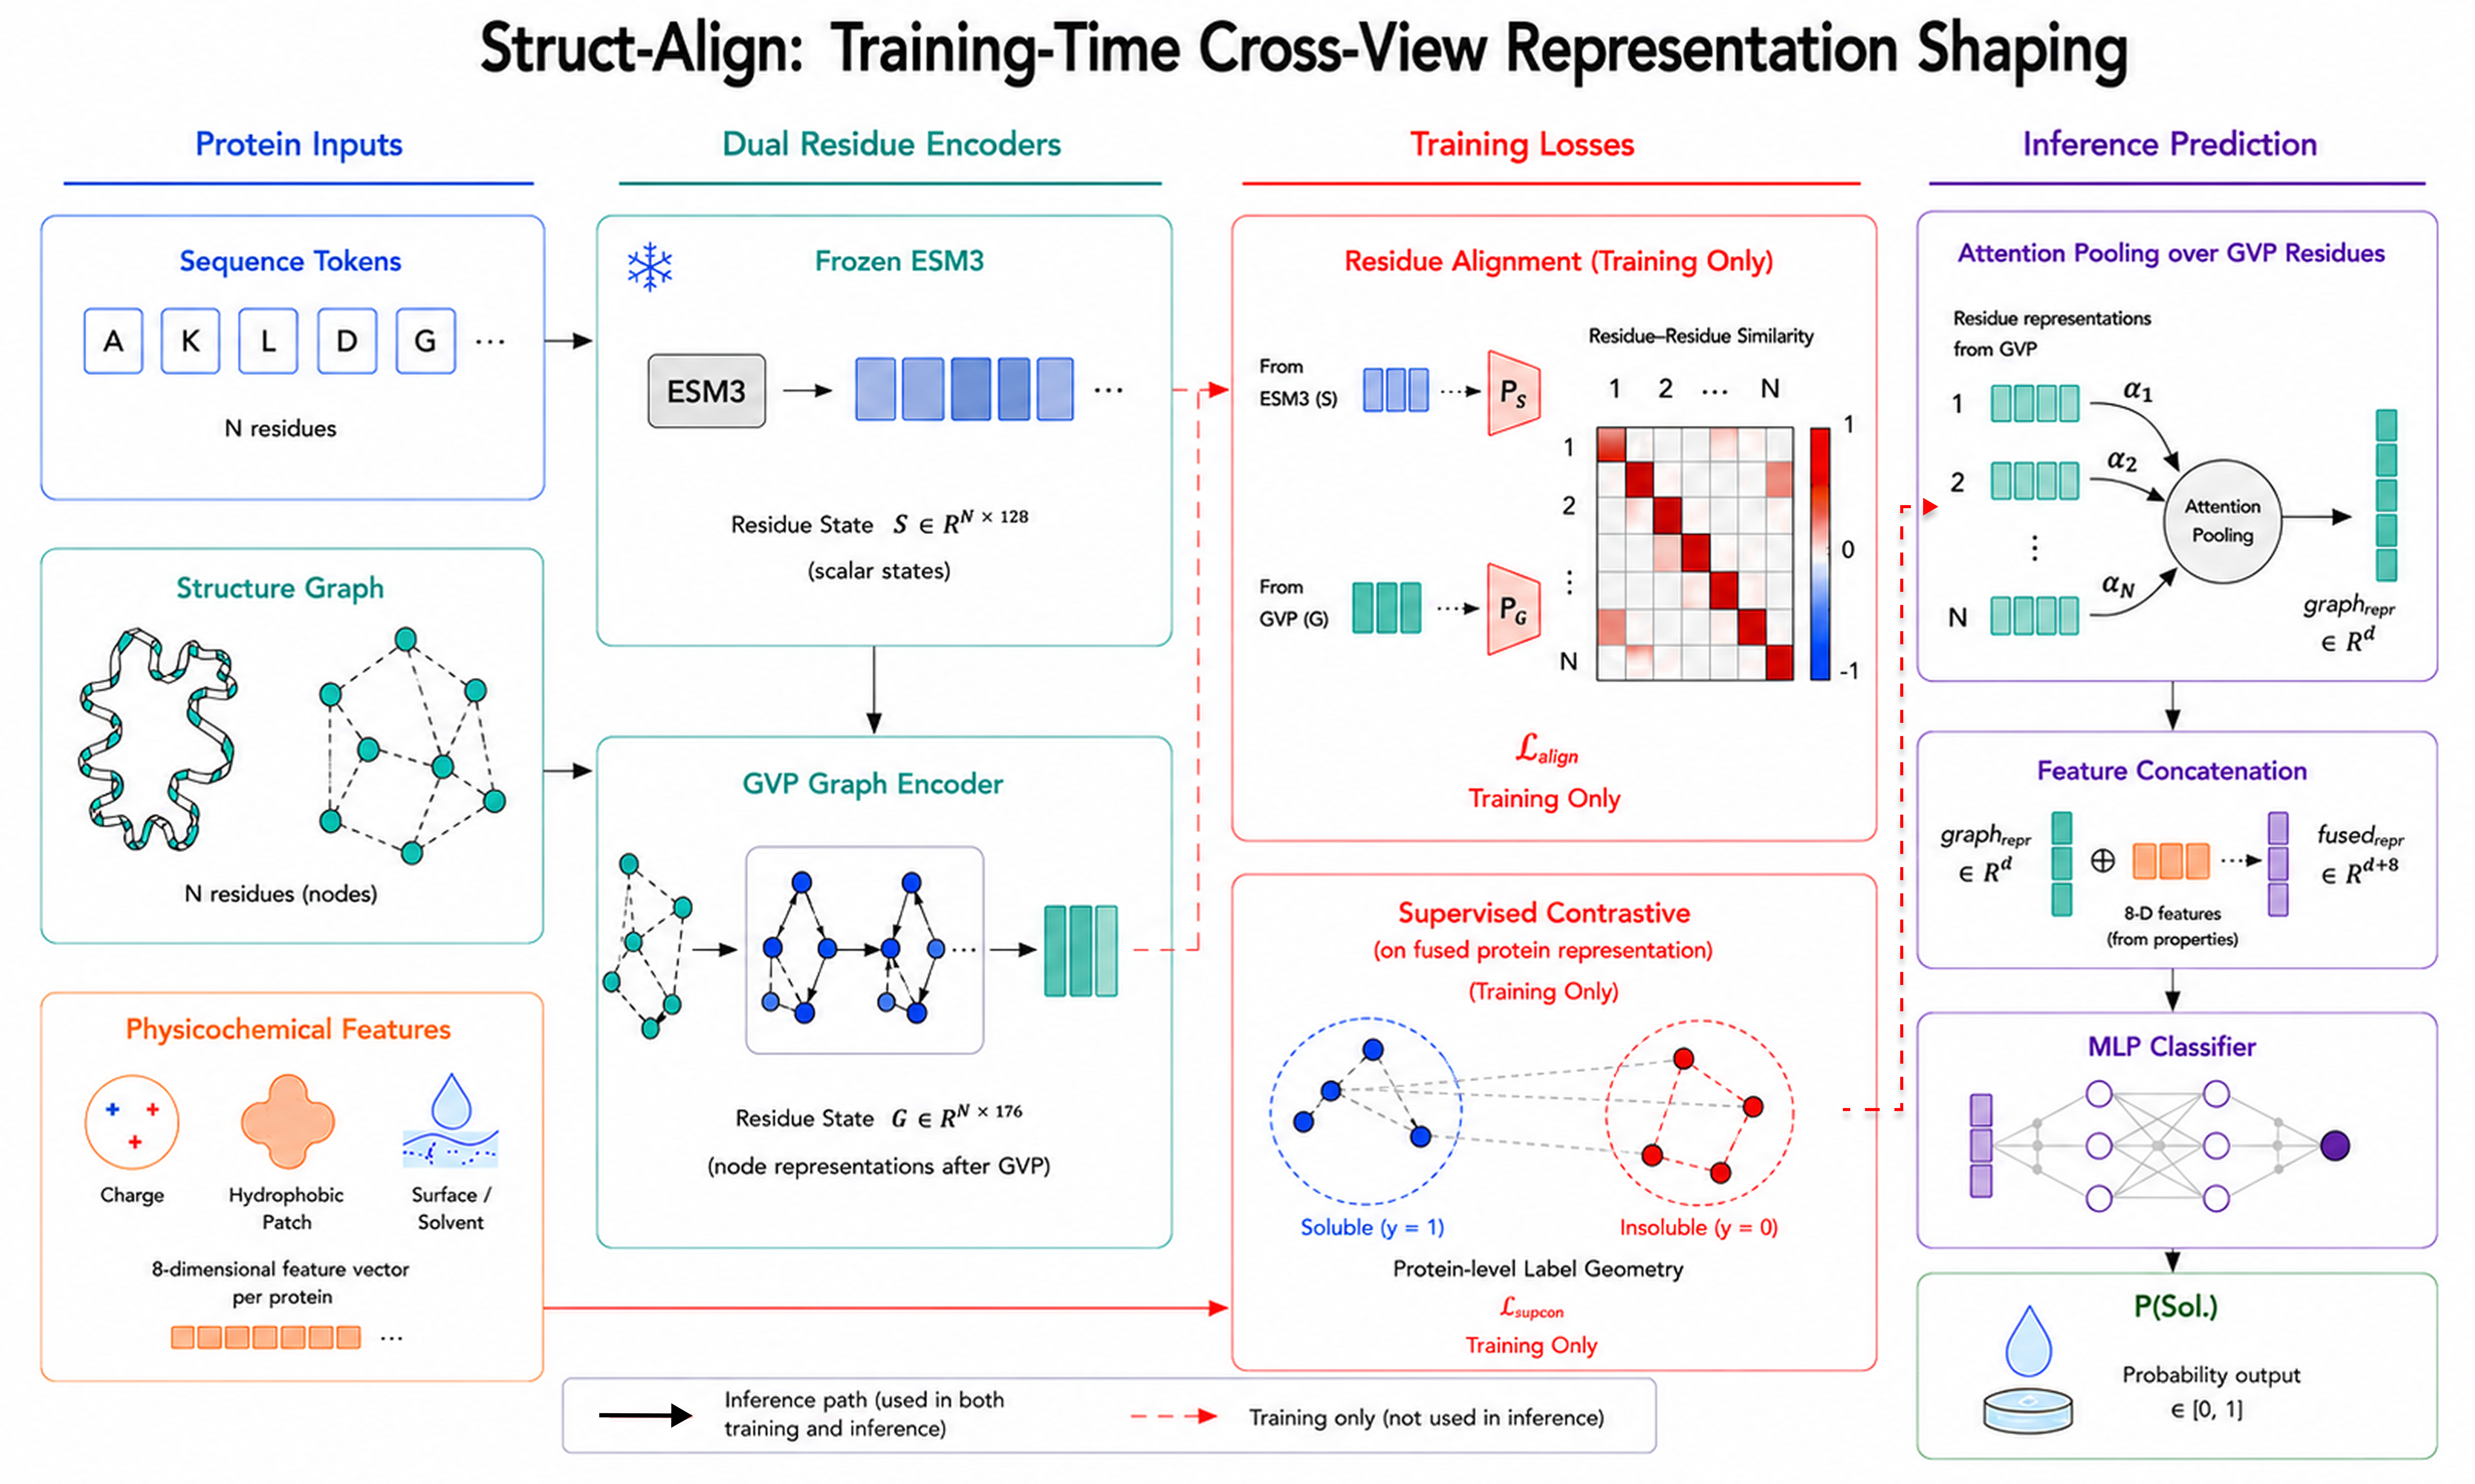
\includegraphics[width=0.96\textwidth]{fig1_workflow.png}
\caption{Overview of Struct-Align. Sequence and structure views are coupled by a residue-level alignment loss used only during training as cross-view consistency regularization. At inference, pooled graph and feature representations are passed to the solubility classifier.}
\label{fig:workflow}
\end{figure*}

\section{Related Work}

\subsection{Protein Solubility Prediction}
Protein solubility prediction has been studied using both hand-crafted descriptors and machine learning. Tools such as CamSol, Protein-Sol, and DeepSol demonstrated that sequence composition, physicochemical descriptors, and neural models can capture useful solubility signals \cite{Sormanni2015,Hebditch2017,Khurana2018}. NetSolP later showed that transformer-based protein language representations can improve soluble expression prediction in \emph{Escherichia coli} under sequence-identity-aware evaluation \cite{Thumuluri2022}.

\subsection{Protein Language and Structure-Aware Models}
Protein language models learn representations from large unlabeled protein sequence corpora. ESM1b and related models established that unsupervised protein sequence learning can encode biological structure and function \cite{Rives2021}. ESM3 further extends protein representation learning with sequence, structure, and function-aware modeling \cite{Hayes2025}. In this work, we use ESM3-open-small as a frozen residue encoder to isolate the effect of structure-aware graph learning and alignment.

Three-dimensional protein structure has been integrated into neural models using residue-contact graphs, equivariant networks, and geometric vector features. GVPs provide a practical way to process scalar and vector features over protein structure graphs \cite{Jing2021}. Structure-aware protein language models such as SaProt also show that residue structure context can improve representation learning \cite{Su2024}. For solubility prediction, methods such as GATSol and ProtSolM motivate the integration of PLM embeddings, structure graphs, and physicochemical features \cite{Tan2024,Li2024}.

\subsection{Contrastive and Multimodal Alignment}
Contrastive learning encourages semantically related representations to be close and unrelated representations to be separated. Supervised contrastive learning uses labels to group examples of the same class \cite{Khosla2020}. Multimodal contrastive alignment has been widely used in vision-language learning and is increasingly relevant for protein modeling. Struct-Align adapts this idea at residue resolution as an auxiliary consistency objective: during training, the positive pair for each residue is its corresponding sequence and structure-conditioned representation in the same protein.

\begin{figure*}[!t]
\centering
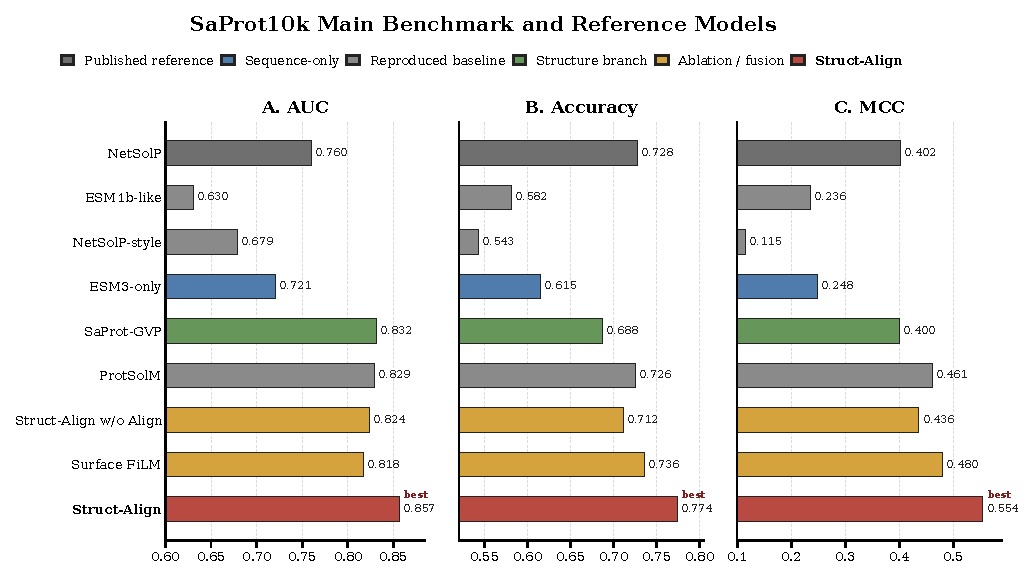
\includegraphics[width=0.86\textwidth]{fig2_saprot10k_results.pdf}
\caption{SaProt10k main benchmark and reference models. Struct-Align achieves the strongest AUC, accuracy, and MCC among the compact set of NetSolP-style, sequence-only, reproduced, structure-branch, ablation, and fusion baselines shown.}
\label{fig:saprot10k}
\end{figure*}

\section{Materials and Methods}

\subsection{Datasets}
The primary benchmark is SaProt10k, a 10,000-protein subset derived from the local SaProt-based solubility dataset used in this study. The prepared benchmark includes protein sequences, binary solubility labels, and structure-compatible fields for downstream graph construction. The main split contains 9,078 training proteins, 714 validation proteins, and 208 test proteins. The overall positive/negative ratio is approximately 42:58, and the mean sequence length is approximately 298.7 residues.

To assess reduced-homology behavior, test proteins were additionally stratified by sequence identity to the training set using MMseqs2-derived identity information \cite{Steinegger2017}. The key low-homology bucket contains 141 test proteins with less than 30\% sequence identity to the training set. We report this subset separately because it better tests whether the model is learning transferable solubility signals rather than relying on close homologs.

External evaluation uses the NetSolP official train/validation/test protocol \cite{Thumuluri2022}. The cleaned protocol file contains 12,549 proteins: 8,283 training, 2,943 validation, and 1,323 test proteins. Because complete experimental structures are not available for all proteins, ESMFold-derived structures are used for structure-aware models \cite{Lin2023}. We treat this setting as an external transfer benchmark with predicted structural inputs rather than an ideal experimental-structure benchmark.

\subsection{Input Representation}
Each protein is represented using three information sources: sequence tokens encoded by ESM3-open-small, residue-level structural graphs constructed from PDB or ESMFold coordinates, and eight-dimensional protein-level physicochemical or surface-related features. The structural graph branch uses residue nodes and geometry-derived edge information. Coordinate masks identify residues with valid structural coordinates. For SaProt10k, available local structure preparation is used. For NetSolP, structures are generated with ESMFold and then converted into SaProt-compatible and graph-compatible inputs.

\subsection{Struct-Align Architecture}
Struct-Align uses ESM3-open-small as the sequence encoder. In the final configuration, ESM3 parameters are frozen. The 1,536-dimensional ESM3 residue embeddings are projected to 128-dimensional node features before graph fusion.

The structural branch uses two GVP convolution layers. The first layer maps scalar/vector node states from $(128,1)$ to $(128,16)$, and the second layer maps $(128,16)$ to $(128,16)$. The resulting graph-aware residue state combines 128 scalar channels and 16 vector channels. Flattening the vector channels gives a 176-dimensional residue representation. For residue-level alignment, the 128-dimensional sequence state and 176-dimensional graph state are linearly projected to a shared 128-dimensional alignment space. Global attention pooling converts residue-level graph states into a protein-level graph embedding.

The final protein representation concatenates the pooled graph embedding with the eight physicochemical or surface-related features. The classifier is a compact feed-forward network:
\begin{equation}
\mathrm{Linear}(184,64) \rightarrow \mathrm{ReLU} \rightarrow \mathrm{Dropout}(0.3) \rightarrow \mathrm{Linear}(64,1).
\end{equation}
The output is a binary solubility logit.

\subsection{Residue-Level Sequence--Structure Alignment}
The core component of Struct-Align is a symmetric residue-level alignment loss. Let $S \in \mathbb{R}^{N \times d}$ be the projected sequence-derived residue representation and $G \in \mathbb{R}^{N \times d}$ be the structure-conditioned graph residue representation for residues with valid coordinates. Both matrices are L2-normalized. A similarity matrix is computed as
\begin{equation}
M = S G^{T}/\tau,
\end{equation}
where $\tau$ is the alignment temperature. The diagonal entries represent matched sequence--structure views of the same residue. Off-diagonal entries represent non-matching residues. The alignment objective applies bidirectional cross-entropy:
\begin{equation}
\mathcal{L}_{align} = \frac{1}{2}\mathrm{CE}(M,\mathbf{y}) + \frac{1}{2}\mathrm{CE}(M^T,\mathbf{y}),
\end{equation}
where $\mathbf{y}$ indexes the diagonal residue correspondence. For long proteins, at most 2,048 valid residues are sampled for the alignment computation to control memory usage. The final setting uses $\tau=0.1$.

\subsection{Training Objective and Evaluation}
The complete objective combines binary cross-entropy, supervised contrastive learning, and residue-level alignment:
\begin{equation}
\mathcal{L} = \mathcal{L}_{BCE} + \lambda_{sup}\mathcal{L}_{SupCon} + \lambda_{align}\mathcal{L}_{align}.
\end{equation}
The final configuration uses $\lambda_{sup}=0.1$ and $\lambda_{align}=0.2$. Supervised contrastive learning is applied to protein-level graph or fused representations so that soluble proteins are encouraged to be closer to soluble proteins and insoluble proteins closer to insoluble proteins.

We report AUC, accuracy, and Matthews correlation coefficient (MCC). Accuracy and MCC use a threshold selected on the validation set and fixed before test evaluation. MCC is emphasized because solubility data are moderately imbalanced. Bootstrap confidence intervals and paired bootstrap tests use 5,000 resamples. The architecture-matched no-alignment ablation is denoted as Struct-Align w/o Align Loss; it retains the GVP graph branch and supervised contrastive regularization but removes $\mathcal{L}_{align}$. To probe whether the learned improvement depends on exact test-time structural correspondence, we evaluate frozen SaProt10k models under structural-view shuffling, random contact rewiring, contiguous block dropout, segment translation, and chain-only graph replacement. We also sweep $\lambda_{align}$ over $\{0,0.05,0.1,0.2,0.5,1.0\}$ to test whether alignment strength changes ranking discrimination and calibrated classification differently. The overall workflow is summarized in Fig.~\ref{fig:workflow}.

\section{Results}

\subsection{Struct-Align Improves SaProt10k Prediction}
The main SaProt10k results are shown in Table~\ref{tab:saprot} and Fig.~\ref{fig:saprot10k}. ESM3-only achieved AUC 0.7205, accuracy 0.6154, and MCC 0.2485, establishing that a frozen ESM3 sequence representation alone is not sufficient for the local solubility benchmark. Reproduced ProtSolM improved substantially, reaching AUC 0.8291, accuracy 0.7260, and MCC 0.4606. GVP+SupCon reached AUC 0.8237, accuracy 0.7115, and MCC 0.4360.

\begin{table}[!t]
\centering
\caption{SaProt10k main benchmark results.}
\label{tab:saprot}
\begin{tabular}{lccc}
\toprule
Model & AUC & Acc. & MCC \\
\midrule
ESM3-only & 0.7205 & 0.6154 & 0.2485 \\
Official-like ESM1b & 0.6305 & 0.5817 & 0.2358 \\
NetSolP-style ESM12 & 0.6788 & 0.5433 & 0.1149 \\
ProtSolM & 0.8291 & 0.7260 & 0.4606 \\
Attn-pool & 0.8240 & 0.6827 & 0.4057 \\
\textbf{Struct-Align} w/o Align Loss & 0.8237 & 0.7115 & 0.4360 \\
SupCon+LayerMix & 0.8005 & 0.7163 & 0.4428 \\
Struct-adapter & 0.7806 & 0.6731 & 0.3571 \\
Cross-attn & 0.8107 & 0.6971 & 0.4311 \\
Surface FiLM & 0.8175 & 0.7356 & 0.4801 \\
\rowcolor{gray!12}\textbf{Struct-Align} & \textbf{0.8565} & \textbf{0.7740} & \textbf{0.5544} \\
\bottomrule
\end{tabular}
\end{table}

Struct-Align produced the strongest main-split SaProt10k result, with AUC 0.8565, accuracy 0.7740, and MCC 0.5544. The bootstrapped 95\% confidence intervals were AUC [0.8025, 0.9052], accuracy [0.7163, 0.8269], and MCC [0.4351, 0.6609]. Compared with ESM3-only, Struct-Align improved AUC by 0.1360 and MCC by 0.3059. Compared with Struct-Align w/o Align Loss, which removes only the explicit residue alignment term while retaining the graph and supervised contrastive components, Struct-Align improved AUC by 0.0328 and MCC by 0.1184. Paired bootstrap testing showed that the improvement over the no-alignment ablation was significant for AUC ($p=0.0436$), accuracy ($p=0.0128$), and MCC ($p=0.0144$). Compared with reproduced ProtSolM, Struct-Align was numerically stronger; this difference was not statistically significant for AUC ($p=0.2276$) or MCC ($p=0.0944$).

\subsection{Low-Homology Evaluation}
The less-than-30\% identity subset contains 141 test proteins. In this subset, Struct-Align reached AUC 0.8326, accuracy 0.7589, and MCC 0.5390. ProtSolM reached AUC 0.7963, accuracy 0.7092, and MCC 0.4261, while Struct-Align w/o Align Loss reached AUC 0.8048, accuracy 0.6950, and MCC 0.4100. These results support the interpretation that Struct-Align is not simply exploiting close homologs in the local benchmark. However, the subset is smaller than the full test set, so it should be interpreted as supportive evidence rather than a complete guarantee against homology-related bias.

\subsection{Ablation Analysis and Alignment-Weight Sensitivity}
\begin{figure*}[!t]
\centering
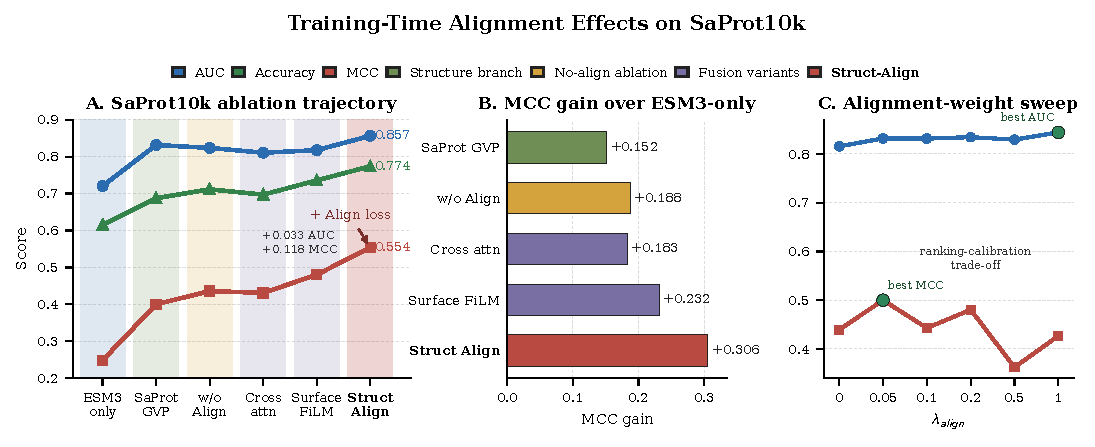
\includegraphics[width=0.96\textwidth]{fig5_ablation_analysis.pdf}
\caption{Ablation and alignment-weight analysis on SaProt10k. Training-time residue-level cross-view consistency improves over the architecture-matched no-alignment model, while the weight sweep shows a ranking--calibration trade-off between AUC and MCC.}
\label{fig:ablation}
\end{figure*}

Fig.~\ref{fig:ablation} and Table~\ref{tab:ablation} summarize the controlled ablation trajectory on SaProt10k. The sequence-only ESM3 baseline reached AUC 0.7205 and MCC 0.2485. Adding a structure-aware graph branch through SaProt-GVP substantially improved AUC to 0.8316 and MCC to 0.4001, indicating that structural context provides useful information beyond frozen ESM3 sequence embeddings. The architecture-matched no-alignment model, Struct-Align w/o Align Loss, further improved calibrated classification over SaProt-GVP, reaching accuracy 0.7115 and MCC 0.4360.

The key ablation is the comparison between Struct-Align and Struct-Align w/o Align Loss. These two models share the same ESM3 backbone, GVP structural branch, graph pooling, supervised contrastive regularization, and classifier; they differ only in whether the residue-level sequence--structure alignment objective is included during training. Adding this objective increased AUC from 0.8237 to 0.8565, accuracy from 0.7115 to 0.7740, and MCC from 0.4360 to 0.5544. The paired bootstrap tests reported above show that these gains are statistically significant, supporting the alignment term as a direct contributor rather than a cosmetic architectural change.

Additional fusion variants did not explain the improvement. Cross-attention reached AUC 0.8107 and MCC 0.4311, while Surface FiLM reached AUC 0.8175 and MCC 0.4801. Surface FiLM improved thresholded metrics relative to the no-alignment model but still remained below Struct-Align, especially in AUC and MCC. This pattern suggests that the main gain is not simply due to adding another fusion module; the training-time residue-level consistency constraint provides a more effective representation-shaping signal.

\begin{table}[t]
\centering
\caption{Ablation summary on SaProt10k.}
\label{tab:ablation}
\begin{tabular}{lccc}
\toprule
Model & AUC & Acc. & MCC \\
\midrule
ESM3-only & 0.7205 & 0.6154 & 0.2485 \\
SaProt-GVP & 0.8316 & 0.6875 & 0.4001 \\
\textbf{Struct-Align} w/o Align Loss & 0.8237 & 0.7115 & 0.4360 \\
Cross-attn & 0.8107 & 0.6971 & 0.4311 \\
Surface FiLM & 0.8175 & 0.7356 & 0.4801 \\
\rowcolor{gray!12}\textbf{Struct-Align} & \textbf{0.8565} & \textbf{0.7740} & \textbf{0.5544} \\
\bottomrule
\end{tabular}
\end{table}

The alignment-weight sweep further supports a regularization interpretation. Nonzero alignment weights improved test AUC over $\lambda_{align}=0$ (0.8154), with the highest AUC at $\lambda_{align}=1.0$ (0.8440). In contrast, threshold-sensitive MCC peaked at a moderate weight (0.5000 at $\lambda_{align}=0.05$) and declined under stronger alignment (0.3623 at $\lambda_{align}=0.5$ and 0.4268 at $\lambda_{align}=1.0$). Thus, increasing alignment strength can preserve or improve ranking discrimination while degrading calibrated classification, suggesting an alignment-induced ranking--calibration trade-off rather than a simple monotonic improvement.

\subsection{External Transfer with Predicted Structures}
Table~\ref{tab:netsolp} shows the NetSolP official-protocol transfer results using ESMFold-derived structural inputs. ESM3-only reached AUC 0.7265, accuracy 0.6931, and MCC 0.2845. ProtSolM reached AUC 0.7653, accuracy 0.7211, and MCC 0.3643. Struct-Align reached AUC 0.7677, accuracy 0.7226, and MCC 0.3680, improving significantly over ESM3-only under paired bootstrap testing (AUC $p<0.001$, MCC $p=0.0020$) and matching ProtSolM within statistical uncertainty (AUC $p=0.8476$, MCC $p=0.9116$).

The no-alignment variant obtained the highest NetSolP score, with AUC 0.7830, accuracy 0.7256, and MCC 0.3961. This result clarifies the operating regime of residue-level alignment: the alignment term is beneficial on SaProt10k, where it significantly improves the architecture-matched ablation, while external transfer may favor a less constrained graph-contrastive objective. We therefore interpret the NetSolP setting as a transfer stress test rather than as primary evidence that inference requires exact residue-level geometric correspondence.

To test the mechanism, we evaluated frozen SaProt10k models under stronger structural-view perturbations. Surprisingly, even complete structural-view reassignment left performance essentially unchanged: full structural-view shuffle yielded AUC 0.8571 and MCC 0.5619, compared with the uncorrupted AUC 0.8565 and MCC 0.5544. Chain-only graph replacement (AUC 0.8610, MCC 0.5562) and 50\% contact rewiring (AUC 0.8571, MCC 0.5812) also preserved performance. These results indicate that the benefit of the alignment objective is primarily realized during representation shaping in training rather than through inference-critical geometric matching.

\begin{table}[t]
\centering
\caption{NetSolP official-protocol results.}
\label{tab:netsolp}
\begin{tabular}{lcccc}
\toprule
Model & AUC & Acc. & MCC & Thr. \\
\midrule
ESM1b-like & 0.6305 & 0.5817 & 0.2358 & -- \\
ESM3-only & 0.7265 & 0.6931 & 0.2845 & 0.310 \\
ProtSolM & 0.7653 & 0.7211 & 0.3643 & 0.600 \\
\rowcolor{gray!12}\textbf{No-align} & \textbf{0.7830} & \textbf{0.7256} & \textbf{0.3961} & 0.640 \\
Struct-Align & 0.7677 & 0.7226 & 0.3680 & 0.605 \\
\bottomrule
\end{tabular}
\end{table}

\subsection{Repeated-Evaluation Summary}
Repeated evaluations provide context for the main split result (Table~\ref{tab:robustness}). The same-split three-seed mean was AUC 0.8227, accuracy 0.7147, and MCC 0.4430. Random five-fold cross-validation produced mean AUC 0.8107 ($\pm$0.0211), accuracy 0.7275 ($\pm$0.0154), and MCC 0.4379 ($\pm$0.0381). These estimates are lower than the strongest main-split result, indicating optimization sensitivity under the current multimodal training configuration. Nevertheless, they remain consistent with the central ablation finding that residue-level alignment improves the architecture-matched SaProt10k baseline.

\begin{table}[t]
\centering
\caption{Struct-Align robustness summary.}
\label{tab:robustness}
\small
\scriptsize
\begin{tabular}{@{}lccc@{}}
\toprule
Setting & AUC & Acc. & MCC \\
\midrule
\rowcolor{gray!12}\textbf{Main split} & \textbf{0.8565} & \textbf{0.7740} & \textbf{0.5544} \\
3 seeds & 0.8227 & 0.7147 & 0.4430 \\
Random CV5 & 0.8107{\scriptsize$\pm$0.0211} & 0.7275{\scriptsize$\pm$0.0154} & 0.4379{\scriptsize$\pm$0.0381} \\
\bottomrule
\end{tabular}
\end{table}

\section{Discussion}
The results support three observations. First, sequence-only ESM3 is not enough for this solubility benchmark. Although ESM3 provides rich contextual representations, its frozen sequence embeddings underperform graph-enhanced and multimodal models. This is consistent with the biological intuition that solubility depends on structural and surface context, not only residue identity and sequence order.

Second, explicit residue-level alignment provides a meaningful gain over an architecture-matched graph contrastive baseline on SaProt10k. Additional probing supports an optimization-regularization interpretation: disrupting structural-view correspondence at inference does not degrade SaProt10k performance, and alignment-strength variation induces a trade-off between ranking refinement and classification calibration. Increasing alignment strength beyond the moderate regime preserved or improved ranking-based discrimination measured by AUC, but degraded threshold-sensitive MCC and accuracy, suggesting that over-weighted alignment alters logit calibration rather than simply reducing representation quality. These findings suggest a sequence-dominant cross-view consistency mechanism: the alignment objective functions primarily as a training-time constraint that regularizes sequence-centered residue representations with a weak structural relational prior, rather than enforcing inference-critical geometric correspondence.

Third, the external NetSolP transfer setting clarifies a boundary condition for the method. Struct-Align remains competitive with ProtSolM and improves over ESM3-only, but the no-alignment graph contrastive variant performs best on NetSolP. Because inference-time structural-view shuffle, contact rewiring, and chain-only replacement do not harm SaProt10k performance, the NetSolP discrepancy is unlikely to be explained by simple geometric noise sensitivity alone. A more plausible explanation is protocol-level distribution shift between SaProt10k and NetSolP, under which the residue-level consistency objective may reinforce dataset-specific cross-view regularities that do not transfer uniformly across benchmarks. This interpretation positions alignment as a useful in-domain representation-shaping objective rather than a universally transferable correction for structural uncertainty. Future versions should consider adaptive alignment weights, dataset-shift-aware calibration, pLDDT-weighted residue masks, and external datasets prepared under harmonized experimental protocols.

The main limitation is that the highest SaProt10k result comes from one main split. The discrepancy between the strongest single-run result and repeated-seed or random-CV averages suggests substantial optimization sensitivity under the current training configuration, likely due to the small held-out test set and multimodal objective balancing. Future work should investigate stabilization through curriculum scheduling, adaptive loss weighting, and larger repeated evaluation protocols. Another limitation is that the work uses computational benchmarks only; experimental wet-lab validation is not available. Finally, the external evaluation currently focuses on NetSolP, whose protocol and label distribution may differ from SaProt10k. Additional datasets prepared under consistent experimental protocols would further define when residue-level alignment is most useful.

\section{Conclusion}
Struct-Align introduces residue-level sequence--structure alignment into a multimodal ESM3-GVP protein solubility predictor. On SaProt10k, the method improves over sequence-only, graph contrastive, and reproduced multimodal baselines, and it retains strong performance in the less-than-30\% identity subset. The controlled no-alignment ablation and paired bootstrap analysis show that explicit residue-level alignment contributes directly to the SaProt10k gain. Stress tests indicate that this gain is realized primarily through training-time cross-view consistency regularization rather than dependence on exact inference-time structural correspondence. External NetSolP transfer remains competitive with ProtSolM but favors the no-alignment variant, suggesting protocol-level distribution shift. Overall, Struct-Align provides a practical representation-shaping framework for structure-informed solubility prediction and motivates future work on shift-aware and externally calibrated multimodal protein learning.

\section*{Code Availability}
Source code and run materials will be released at \url{https://github.com/AAAYONG-1113/Struct-Align-Residue-Level-Cross-View-Consistency-Regularization-for-Protein-Solubility-Prediction}.

\begin{thebibliography}{99}

\bibitem{Sormanni2015}
P. Sormanni, F. A. Aprile, and M. Vendruscolo, ``The CamSol method of rational design of protein mutants with enhanced solubility,'' \emph{J. Mol. Biol.}, vol. 427, pp. 478--490, 2015.

\bibitem{Hebditch2017}
M. Hebditch, M. A. Carballo-Amador, S. Charonis, R. Curtis, and J. Warwicker, ``Protein-Sol: a web tool for predicting protein solubility from sequence,'' \emph{Bioinformatics}, vol. 33, pp. 3098--3100, 2017.

\bibitem{Khurana2018}
S. Khurana, R. Rawi, R. Kunji, G. Y. Chuang, H. Bensmail, and R. Mall, ``DeepSol: a deep learning framework for sequence-based protein solubility prediction,'' \emph{Bioinformatics}, vol. 34, pp. 2605--2613, 2018.

\bibitem{Thumuluri2022}
S. Thumuluri, H. M. Martiny, J. A. Almagro Armenteros, J. Salomon, H. Nielsen, and A. R. Johansen, ``NetSolP: predicting protein solubility in \emph{Escherichia coli} using language models,'' \emph{Bioinformatics}, vol. 38, pp. 941--946, 2022.

\bibitem{Rives2021}
A. Rives \emph{et al.}, ``Biological structure and function emerge from scaling unsupervised learning to 250 million protein sequences,'' \emph{Proc. Natl. Acad. Sci. USA}, vol. 118, e2016239118, 2021.

\bibitem{Hayes2025}
T. Hayes \emph{et al.}, ``Simulating 500 million years of evolution with a language model,'' \emph{Science}, vol. 387, pp. 850--858, 2025.

\bibitem{Jumper2021}
J. Jumper \emph{et al.}, ``Highly accurate protein structure prediction with AlphaFold,'' \emph{Nature}, vol. 596, pp. 583--589, 2021.

\bibitem{Lin2023}
Z. Lin \emph{et al.}, ``Evolutionary-scale prediction of atomic-level protein structure with a language model,'' \emph{Science}, vol. 379, pp. 1123--1130, 2023.

\bibitem{Jing2021}
B. Jing, S. Eismann, P. Suriana, R. J. L. Townshend, and R. O. Dror, ``Learning from protein structure with geometric vector perceptrons,'' in \emph{Proc. ICLR}, 2021.

\bibitem{Tan2024}
Y. Tan, J. Zheng, L. Hong, and B. Zhou, ``PROTSOLM: Protein solubility prediction with multi-modal features,'' in \emph{Proc. IEEE BIBM}, pp. 223--232, 2024.

\bibitem{Li2024}
B. Li and D. Ming, ``GATSol, an enhanced predictor of protein solubility through the synergy of 3D structure graph and large language modeling,'' \emph{BMC Bioinformatics}, vol. 25, p. 204, 2024.

\bibitem{Su2024}
J. Su, C. Han, Y. Zhou, J. Shan, X. Zhou, and F. Yuan, ``SaProt: Protein language modeling with structure-aware vocabulary,'' in \emph{Proc. ICLR}, 2024.

\bibitem{Khosla2020}
P. Khosla \emph{et al.}, ``Supervised contrastive learning,'' in \emph{Advances in Neural Information Processing Systems}, vol. 33, pp. 18661--18673, 2020.

\bibitem{Steinegger2017}
M. Steinegger and J. Soeding, ``MMseqs2 enables sensitive protein sequence searching for the analysis of massive data sets,'' \emph{Nat. Biotechnol.}, vol. 35, pp. 1026--1028, 2017.

\end{thebibliography}

\end{document}
